%--------------------------------
%--------------------------------
\chapter{Implementierungsdetails}
\label{chapter_implementation_detail}

%---------------------------
\section{Programmiersprache}

\begin{itemize}
 \item Rust: nicht geeignet, da Datenstrukturen die zyklische Referenzen auf veränderbare Objekte verwenden nicht oder nur kompliziert umsetzbar sind.
 \item Java: scheint gut zu funktionieren. Es gibt Bibliotheken zum im-/exportieren von obj-Dateien und Unterstützung für OpenGL
\end{itemize}


%---------------------
\section{Dateiformate}

\begin{itemize}
 \item Einfachstes Format (nur für die Darstellung von 3D-Objekten ohne Zusatzinformationen): obj
 \item Erster Schritt: einfaches .obj erzeugen und mit Blender darstellen; einfach Knochen als Bounding Box darstellen
 \item Jeder Editor geht mit Muskeln und Gelenken anders um. Gibt es ein Dateiformat, das nicht speziell zu einem Editor gehört, dass Bedingungen an die Rotation von Gelenken speichern kann?
 \item Eigenes Format erzeugen? Dann bräuchte man Plugins um es in verschiedenen Editoren laden zu können. Viel verwendeter Editor: Houdini (kostenlos für Studenten aber nicht Open Source). Oder selbst darstellen (siehe Interaktivität).
\item Vorschlag von Jo: "`Memory dumps"', also direkt die structs aus dem speicher auf platte rausschreiben. Am besten wenn sie am Stueck liegen mit einem fwrite() und zurücklesen mit einem fread(). Es ist nuetzlich dazu am Anfang der Datei ein bisschen Metadaten zu speichern (magic number, version, array size etc).
\end{itemize}

%- - - - - - - - - -
\subsection{OpenSim}

\begin{itemize}
 \item \url{https://simtk-confluence.stanford.edu:8443/display/OpenSim/OpenSim+Documentation}
 \item Open Source Software Platform für die Modellierung uns Simulation von Menschen, Tieren, etc.\\
 aber vor allem gedacht zur Auswertung von experimentellen Daten
 \item Import von .obj Dateien möglich. Außerdem zusätzliche Daten wie Winkel von Gelenken über .mot oder .sto Dateien (eigenes Format von OpenSim, siehe \url{https://simtk-confluence.stanford.edu:8443/display/OpenSim/Preparing+Your+Data})
 \item Export in andere Dateiformate nicht möglich (?)
 \item für Download und Zugang zur "`Community"' Account nötig
 \item für Windows und Mac OS (Linux Support gibt es auch, ist aber schwieriger: \url{https://simtk-confluence.stanford.edu:8443/display/OpenSim/Linux+Support})
\end{itemize}


%- - - - - - - -
\subsection{OBJ}

\begin{itemize}
 \item Beschreibung des Formats: \url{https://www.fileformat.info/format/wavefrontobj/egff.htm}
 \item Erzeugung mit Rust: obj\_exporter \url{https://docs.rs/obj-exporter/0.2.0/obj_exporter/index.html}
 \item Erzeugung mit Java: javagl Obj \url{https://github.com/javagl/Obj}, unterstützt auch Umwandlung von obj-Daten in Daten, die direkt für vertex buffer objects in OpenGL verwendet werden können
 \item Reicht wahrscheinlich für die ersten Dinge aus. Finetuning wird sowieso mit anderer Software gemacht
\end{itemize}

%- - - - - - - -
\subsection{FBX}

\begin{itemize}
 \item Verwendung am besten über Autodesk FBX SDK für C++. 
 \item Dokumentation: \url{http://help.autodesk.com/view/FBX/2019/ENU/} und \url{http://docs.autodesk.com/FBX/2014/ENU/FBX-SDK-Documentation/index.html}
 \item Es gibt auch fbxcel, eine FBX library für Rust. Ist aber relativ low level und nicht ganz offensichtlich wie zu verwenden.
 \item Einschränkungen für Gelenke können in FBX nicht gespeichert werden \url{http://docs.autodesk.com/FBX/2014/ENU/FBX-SDK-Documentation/index.html?url=cpp_ref/class_fbx_constraint.html,topicNumber=cpp_ref_class_fbx_constraint_htmlc57a3f99-513a-44a0-a24f-445e9077c99f}
\end{itemize}

%- - - - - - - - - -
\subsection{Alembic}

\begin{itemize}
 \item \url{www.alembic.io}
 \item Wird u.a. dafür verwendet Knochen (+ Animationen) in Ziva zu importieren
 \item Es kann mit Python (PyAlembic) und C++ verwendet werden.\\
 PyAlembic Doku: \url{http://docs.alembic.io/python/examples.html#pyalembic-intro}\\
 C++ API Refernce (enthält sehr wenig Infos): \url{http://docs.alembic.io/reference/index.html}
 \item Für Rust gibt es keine Bibliothek (?)
\end{itemize}


%-----------------------
\section{Interaktivität}

\begin{itemize}
 \item OpenGL
 \begin {itemize}
  \item SDL + OpenGL Tutorials \\ \url{http://headerphile.com/sdl2/opengl-part-1-sdl-opengl-awesome/}, \\ \url{http://www.sdltutorials.com/sdl-opengl-tutorial-basics}
  \item Daten direkt mit OpenGL erzeugen (laden als vertex und index array)
 \end {itemize}

 \item Benutzeroberfläche
 \begin{itemize}
  \item imgui (opengl/vulcan/3D view integriert) mit Rust oder C++: \url{https://github.com/ocornut/imgui}
  
  \begin{itemize}
   \item OpenGL und Imgui für Rust: \url{https://nercury.github.io/rust/opengl/tutorial/2018/02/08/opengl-in-rust-from-scratch-00-setup.html}, \url{https://github.com/michaelfairley/rust-imgui-sdl2}
   \item es gibt Java Bindings (\url{https://github.com/ice1000/jimgui}), aber Swing ist wahrscheinlich einfacher
   \item OpenGL scene $\rightarrow$ imgui: \url{https://gamedev.stackexchange.com/questions/140693/how-can-i-render-an-opengl-scene-into-an-imgui-window}
  \end{itemize}

  
  \item Java Swing Bibliothek und JOGL (Java OpenGL Binding) (\url{http://www.jogl.info})
 \end{itemize}
\end{itemize}

%-----------------------------
\section{Technische Umsetzung}

\begin{itemize}
 \item Repräsentation des Zustands als Hierarchie von einzelnen Komponenten (terminale sowie nichtterminale).
 \item Übersetzung in ein 3D-Modell: zunächst .obj, später Verwendung von OpenGL mit vertex shadern etc.\
 \item linearer Kongruenzgenerator reich für Zufallszahlen aus, da nur wenige erzeugt werden (erkennbare Muster entstehen erst bei mehr Zufallszahlen) (erwähnen?)
 \item Um Wirbelsäule aus PCA Daten differenzierbar zu machen, wurden jeweils der vorletzte und der zweite Punkt von Hals und Rücken \bzw Rücken und Schwanz um den Kontaktpunk um den gleichen Winkel in gegensätzliche Richtungen gedreht, damit beide Bézierkurven an dem Kontaktpunkt die gleiche Steigung haben. \todo{beste Lösung?}
\end{itemize}

%--------------------------------
\section{Transformationsmatrizen}

Jedes Element im Skelett speichert, relativ zu seinem Elternelement, die Position des Ursprungs seines Koordinatensystems. Um den Überblick über die Transformationsmatrizen bzw. Abbildungen behalten, die vom einen ins andere Koordinatensystem umwandeln, hier zwei Übersichtsgrafiken:

\begin{figure}
 \centering
 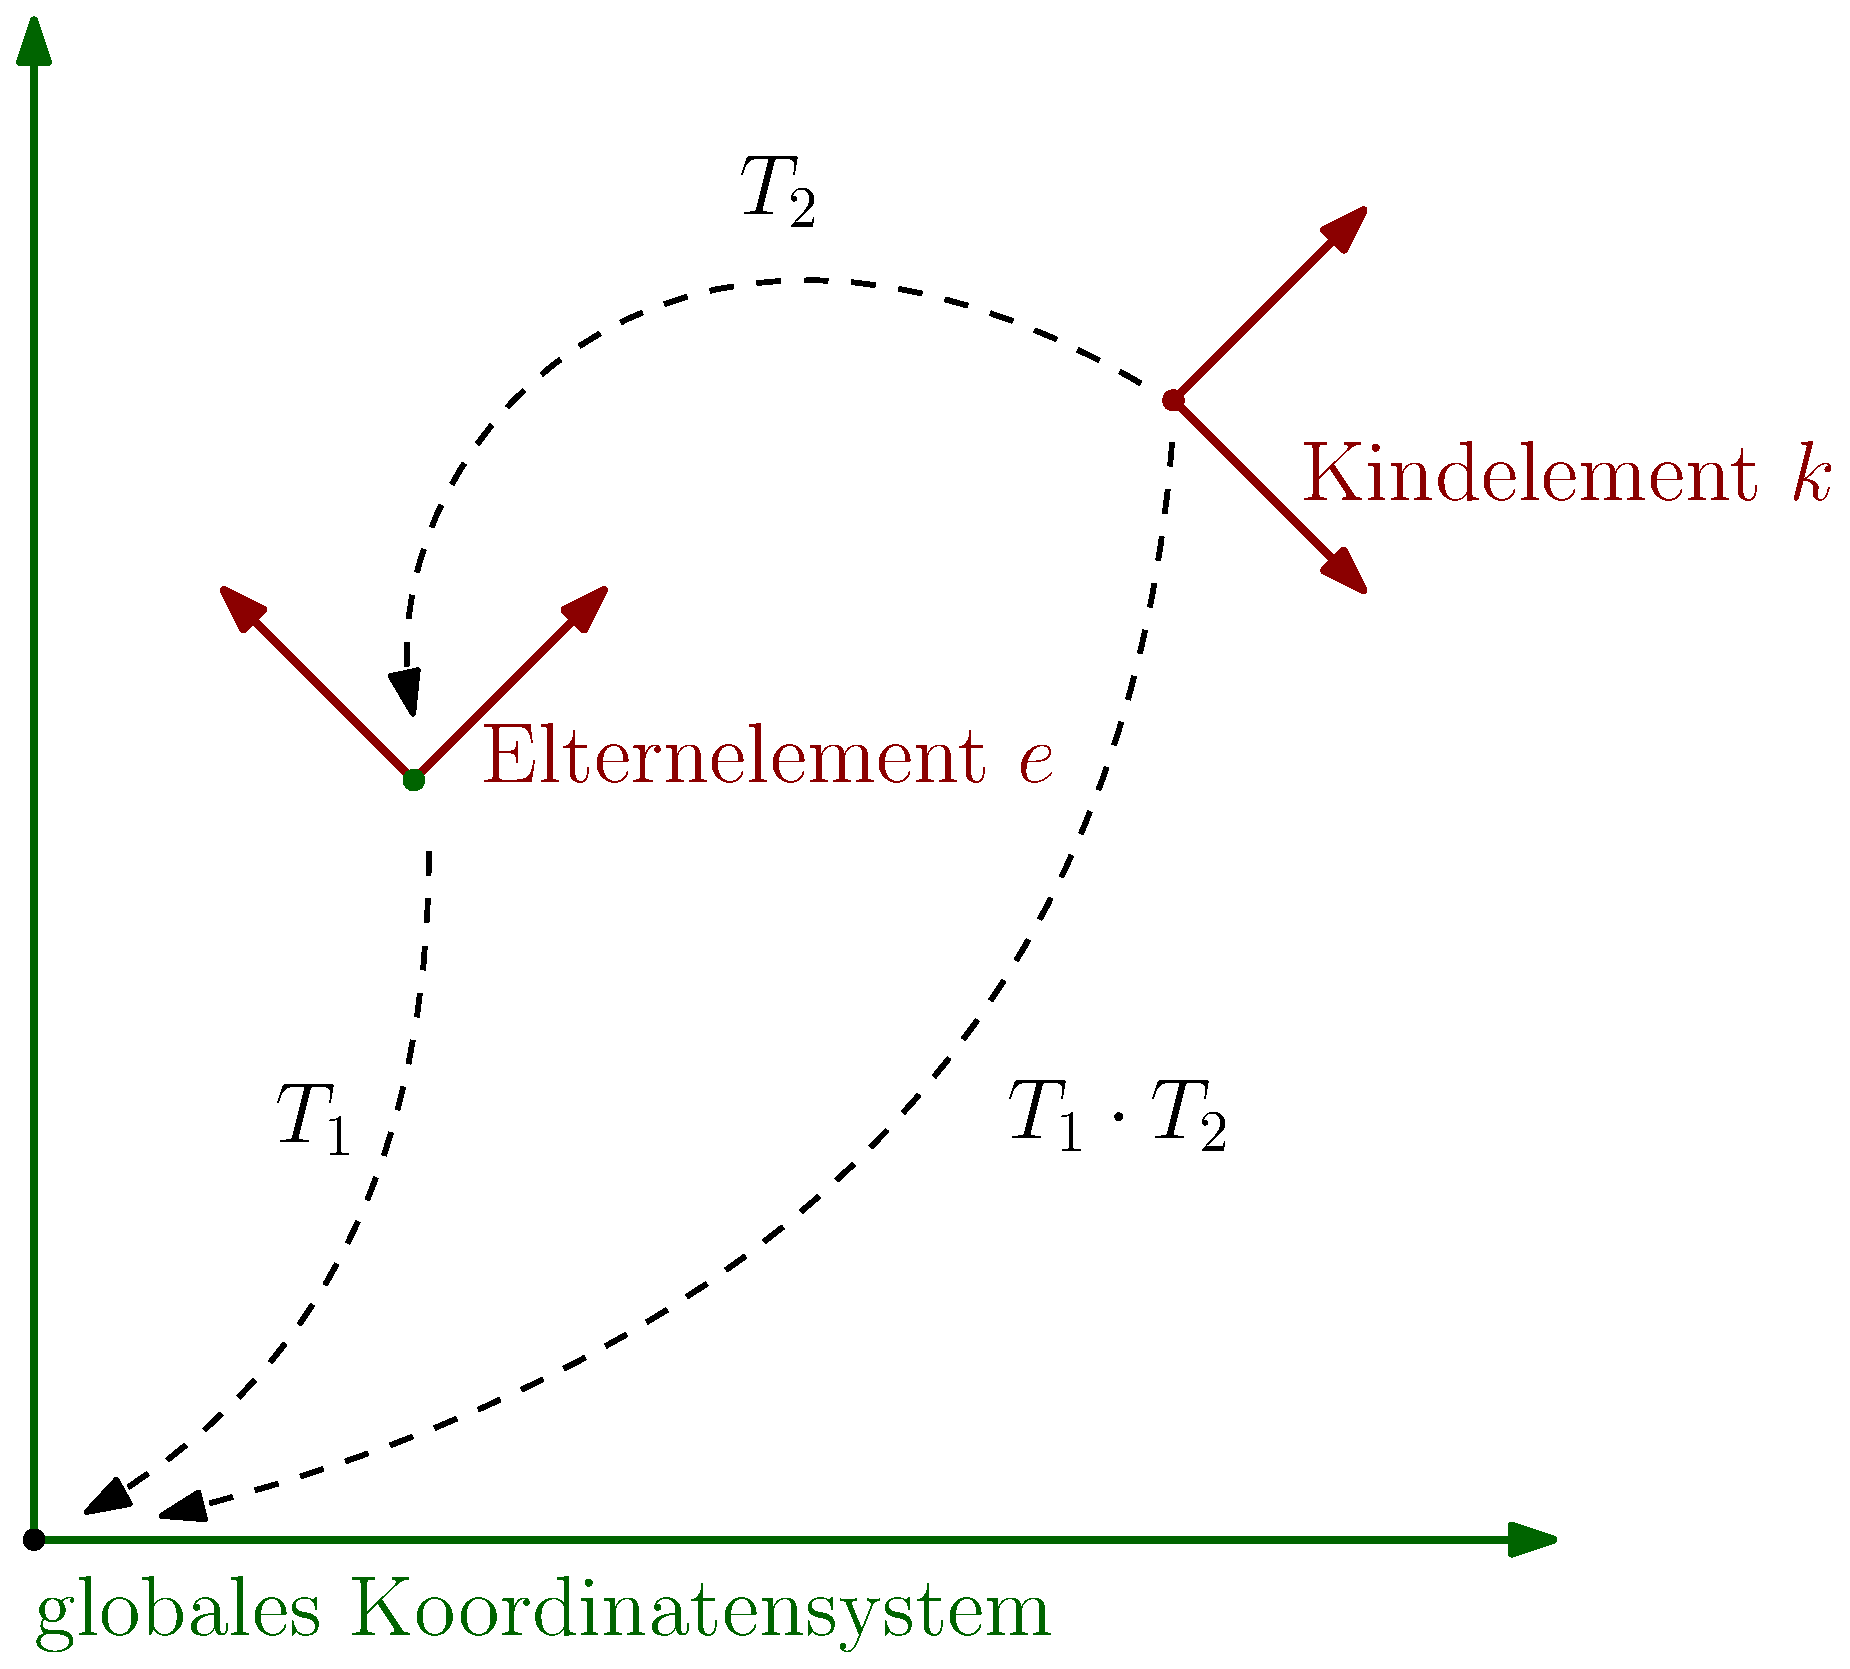
\includegraphics[width=0.6\textwidth]{graphics/transformation_matrices.eps}
 \caption{Gegeben sei das Element $e$. Die Abbildung, die die lokalen Koordinaten von $e$ in globale Koordinaten umrechnet sei $T_1$.
 Jedes Kindelement $k$ von $e$ speichert eine Transformationsmatrix $T_2$, die angibt wo der Ursprung des Koordinatensystems von $k$ relativ zum Koordinatensystem von $e$ liegt. Will mann nun Koordinaten von $k$ in globale Koordinaten umrechnen, benötigt man die Abbildung $T_1 \cdot T_2$.}
\end{figure}

\begin{figure}
 \centering
 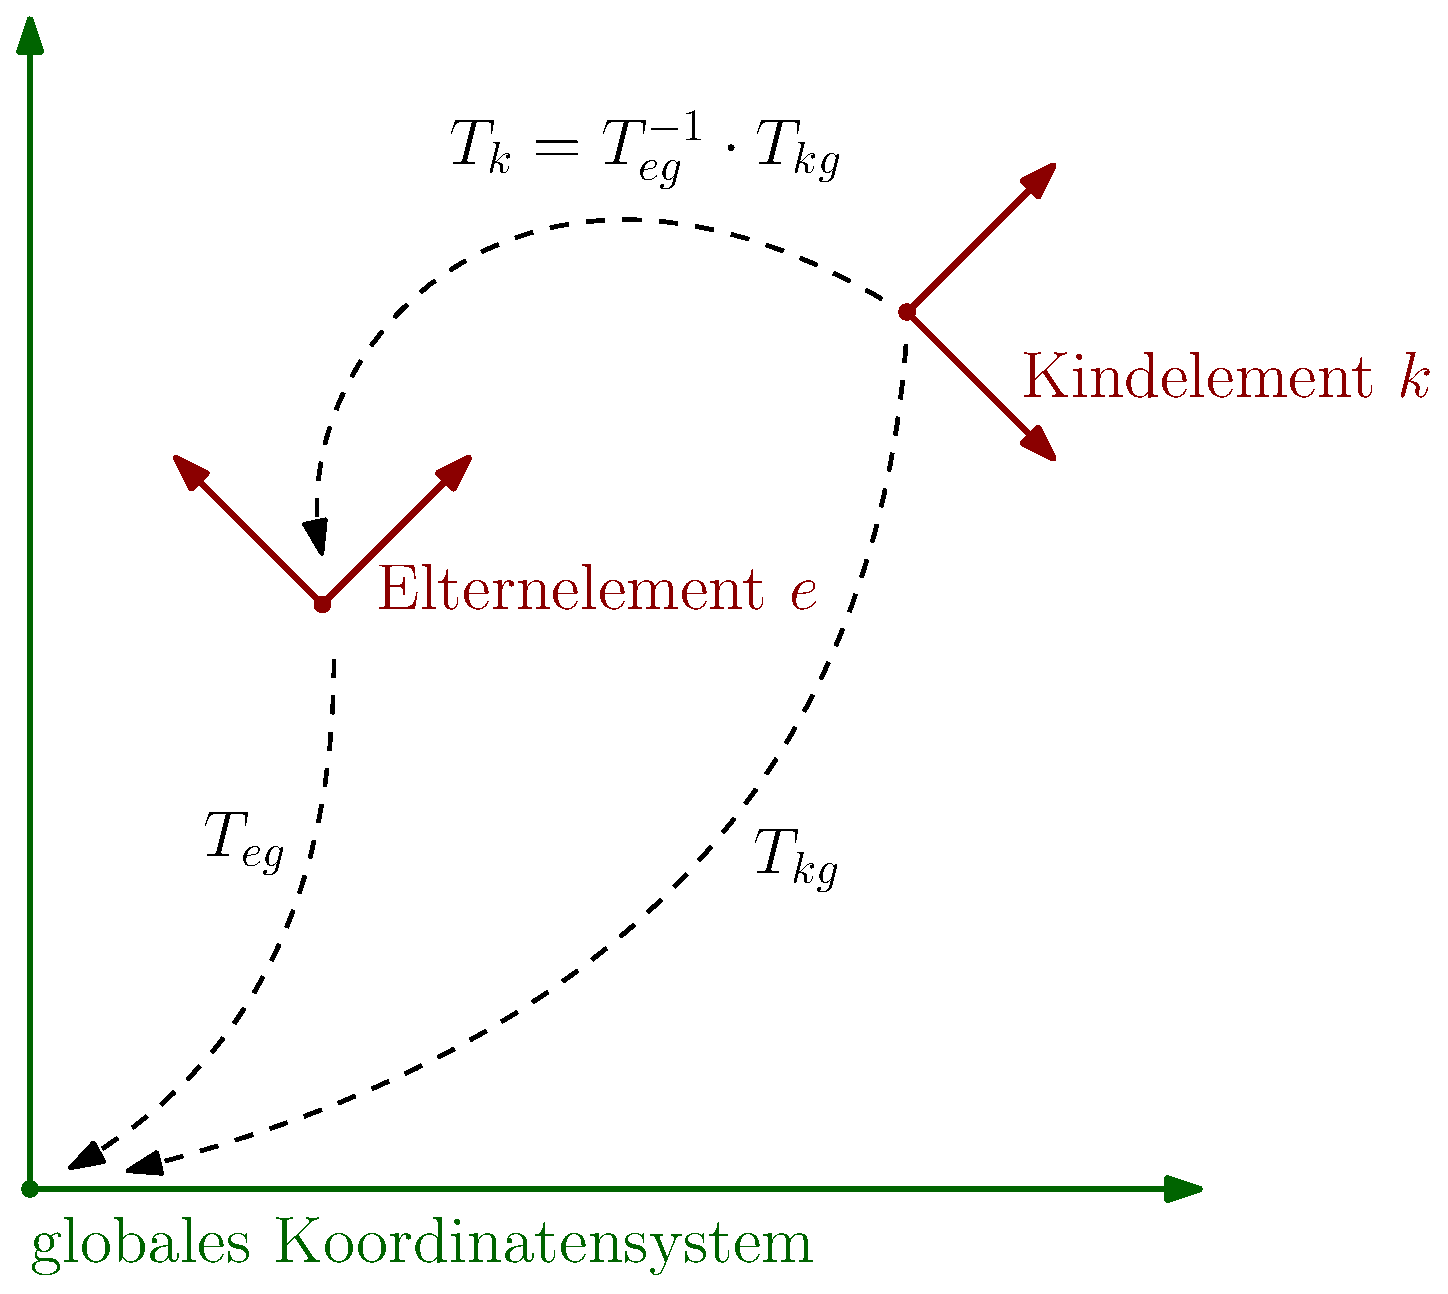
\includegraphics[width=0.6\textwidth]{graphics/transformation_matrices_spine.eps}
 \caption{Will man ein Element $k$ erzeugen, das Kindelement von $e$ ist und dessen globale Koordinaten bekannt sind, muss man die Abbildung berechnen, die die relative Position von $k$ angibt. Seien $T_1$ und $T_2$ jeweils die Transformationen in das globale Koordinatensystem von $e$ \bzw $k$. Dann ist die gesuchte Abbildung $T_1^{-1} \cdot T_2$.}
\end{figure}


%------------
\section{PCA}
\label{section_pca}
%- - - - - - - - - - - - - - - - -
\subsection{Annotation der Bilder}

Die Annotation der Bilder wurde per Hand mit dem Programm Inkscape\footnote{Programm zum erstellen und bearbeiten von Vektorgrafiken, \url{https://inkscape.org/de}} durchgeführt. Für jedes zu markierende Element wurde eine Strecke oder eine Bézierkurve eingefügt und mit einem vorher festgelegten Namen benannt. Diese Elemente wurden dann durch Inkscape als Pfade in der erzeugten svg-Datei gespeichert. Aus dieser Datei wurden dann automatisiert die eingetragenen Pfade mit ihren Koordinaten ausgelesen.

Folgende Details sind wichtig zu beachten, damit dieser Vorgang reibungslos abläuft. 
\begin{itemize}
 \item Man kann in Inkscape einstellen, dass Koordinaten immer absolut angegeben werden. Das ist sinnvoll um die Koordinaten leichter auslesen zu können.
 \item Der Ursprung des Koordinatensystems in Inkscape ist unten links, im svg-Format ist er aber oben links.
 \item Ebenen sollten in Inkscape nicht verschoben sein, sonst verschieben sich mit ihnen auch die Koordinaten.  
\end{itemize}

%- - - - - - - - - - - - - - - - - - - - - - - - - - - - - - - -
\subsection{Anpassung der PCA-Ergebnisse zur Weiterverarbeitung}

\begin{itemize}
 \item An den Kontakpunkten der Wirbelsäulenteile ist die Steigung nicht unbedingt gleich (die Wirbelsäule als ganzes ist nicht $C^1$). Deshalb müssen vor der Weiterverwendung die jeweils nächsten Kontrollpunkte nach dem Kontakpunkt verschoben werden. Das wurde hier so gemacht, dass die zu verschiebenden Kontrollpunkte um den Kontakpunkt in gegensätzliche Richtungen rotiert wurden. Beide werden um den gleichen Winkel rotiert (siehe Abbildung \ref{smooth_spine}). Grundsätzlich könnten die Kontrollpunkte beliebig auf der Tangente des Kontaktpunkts platziert werden (rot im Bild) um eine übereinstimmende Steigung zu bekommen. Um den Verlauf der Wirbelsäulenteile möglichst wenig zu verändern ist es von Vorteil auch die Kontrollpunkte möglichst wenig zu verschieben. Man könnte die Punkte \zb auch senkrecht auf die Tangente projizieren. Welches Verfahren angewendet wird, ist jedoch nicht von großer Bedeutung. 
\end{itemize}

\begin{figure}
 \subfloat[vorher]{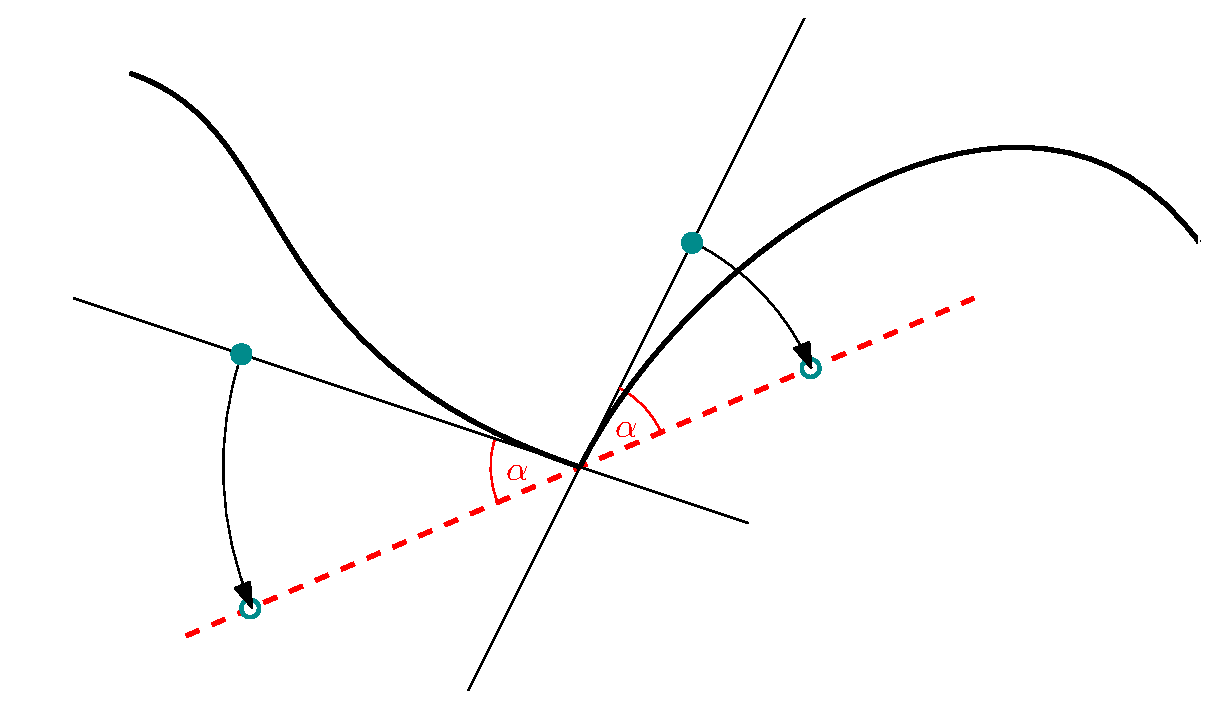
\includegraphics[width=0.5\textwidth]{graphics/smooth_spine1.eps}}
 \qquad
 \subfloat[nachher]{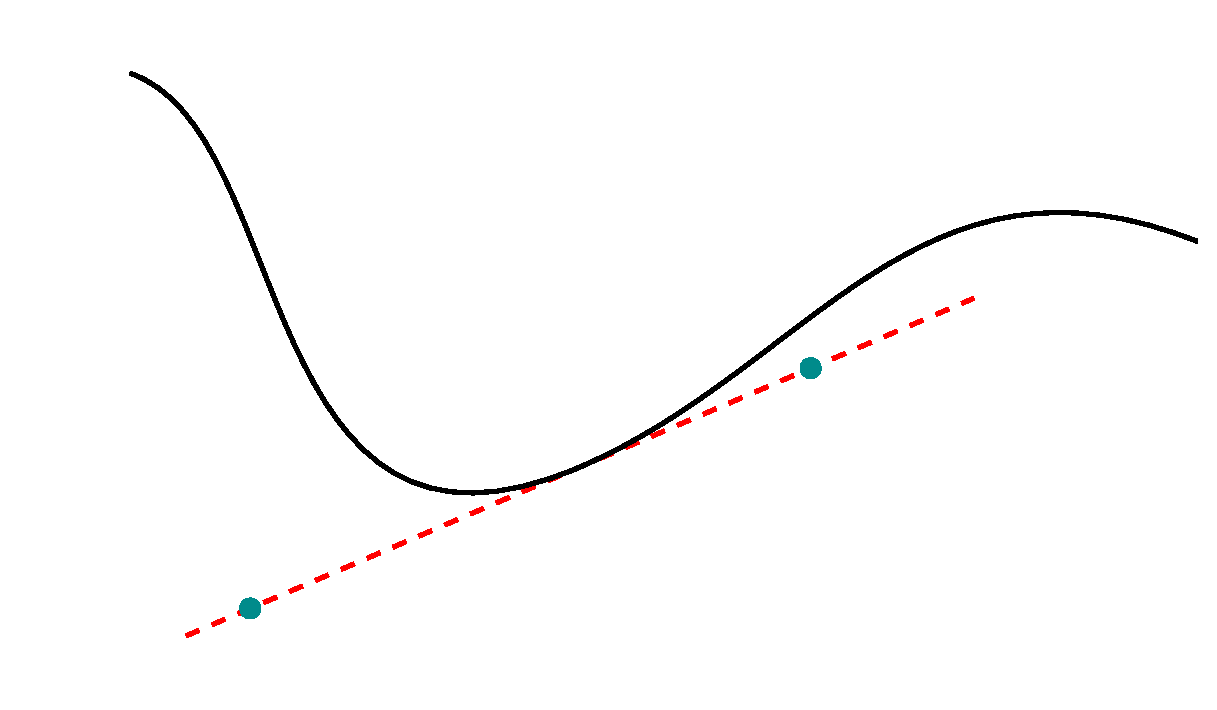
\includegraphics[width=0.5\textwidth]{graphics/smooth_spine2.eps}}
 \caption{Anpassung der Kontrollpunkte der Wirbelsäulenteile, wenn die Steigung an den Kontakpunkten ungleich ist. Die beiden Teile der Wirbelsäule und die Steigung am Kontaktpunkt sind hier in schwarz dargestellt. Die zu drehenden Kontollpunkte in cyan. In rot ist die resultierende Steigung und der Winkel, der für die Drehung verwendet wird, zu sehen.}
 \label{smooth_spine}
\end{figure}




